\documentclass{article}
\usepackage{wasysym}
\usepackage{textcomp}
\usepackage{tikz}

\newcommand{\crel}{
	\hspace{-.6em}
	\begin{tikzpicture}[baseline={([yshift=-.8ex]current bounding box.center)}]
		\draw [->] (0,0) -- (0.45,0); 
		\draw [fill] (0.5,0) circle (0.05);
	\end{tikzpicture}
	\hspace{-.6em}
}

\newcommand{\rrel}{
	\hspace{-.6em}
	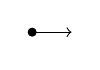
\begin{tikzpicture}[baseline={([yshift=-.8ex]current bounding box.center)}]
		\draw [fill] (0,0) circle (0.05);
		\draw [->] (0.05,0) -- (0.5,0);
	\end{tikzpicture}
	\hspace{-.6em}
}

\newcommand{\mrel}{
	\hspace{-.6em}
	\begin{tikzpicture}[baseline={([yshift=-.8ex]current bounding box.center)}]
		\draw [->] (0,0) -- (0.4,0);
		\draw (0.4,0) -- (0.475,0.075) -- (0.55,0) -- (0.475,-0.075) -- cycle;
	\end{tikzpicture}
	\hspace{-.6em}
}

\newcommand{\irel}{
	\hspace{-.6em}
	\begin{tikzpicture}[baseline={([yshift=-.8ex]current bounding box.center)}]
		\draw [->] (0,0) -- (0.4,0);
		\draw (0.41,0) -- (0.55,0);
		\draw (0.48,-0.07) -- (0.48, 0.07); 
	\end{tikzpicture}
	\hspace{-.6em}
}

\newcommand{\erel}{
	\hspace{-.6em}
	\begin{tikzpicture}[baseline={([yshift=-.8ex]current bounding box.center)}]
		\draw [->] (0,0) -- (0.4,0);
		\draw (0.41,0) -- (0.55,0);
		\draw (0.48, 0.05) circle (0.02);
		\draw (0.48, -0.05) circle (0.02); 
	\end{tikzpicture}
	\hspace{-.6em}
}

\begin{document}
	\section*{Framework}
	\textbf{Failure model}: Byzantine failures with subsystems exhibiting only crashes (no key guessing)\\
	\noindent
	Workflow: $G=(V,E)$ \\
	Activities: $V=\{v_1,\ \dots, v_n\}$ \\ %missing event states
	Activity States: $S=\{s_1,\ \dots, s_n\}$, where $s_i \subseteq \{Executed, Pending, Included\}$\\
	Relation ($E$): $R=($condition, response, milestone, include, exclude$)$, $e=(v_x, v_y, r_i)$, $E=\{e_1,\ \dots, e_m\}$\\
	Actors: $P =\{$Alice ($A$), Bob ($B$)$\}$.\\ %(Deciders vs. witnesses)
	History, $H_A(t)$, $H_B(t)$: Sequence of activity executions up to, and at time $t$, as perceived by $A$ and $B$, respectively.\\
	Execution: $(v_i, t, p_i)$, where $v_i$ is the activity executed at time $t$, executed by actor $p_i$.\\
	%History, $H(t)$: State of the entire workflow at time $t$

	\section*{Problem}
	Ensure that two parties collaborating on a DCR graph, can execute the activities in the graph without requiring any degree of trust. We want to ensure fairness in the sense that each collaborator will be able to execute their relevant activities (in so far as they can do so according to the specific DCR graph), and that no collaborator can repudiate executions of activities (neither their own nor other parties').
	The resulting global state of the distributed executions must be a result of a valid execution sequence in the workflow.

	1. There must be a happened-before relationship between an execution and the executions of its dependent activities
	2. All serializations of the happened-before relationships must be valid execution sequences in DCR

	\section*{Requirements}
	\begin{description}
		\item[Consensus]:
			\begin{description}
				\item[Termination] Eventually each correct process sets its decision value (single activity state)
				\item[Agreement] Decision vector = activity state
								1. Eventual agreement: We can poll for an history, after which agreement on current state is reached.
								2. Partial agreement: Bottom is allowed as substitute for any activity state (not if you're responsible for that activity)
				\item[Integrity] If $p_i$ is correct, then all correct processes decide on $v_i$, or $\bot$ as the ith component of their vector.
			\end{description}
		\item[Concurrency]: DCR-rules for concurrency (only independent activities can be concurrent) (Tie-breaking)
		\item[Correctness]: The system must enforce the agreed-upon workflow, so that no party can obtain an advantage by acting out of turn or failing to fulfil an obligation to act.
		\item[Non-repudiation]: $v_i$ must be provably proposed by $p_i$, within a negligible probability.
		% \item[Co-non-repudiation?]:
	\end{description}

	\section*{Scenarios}
	\begin{description}
		\item[Scenario 1] 
			$A\crel B$\\
			Alice must never decide $\bot$ for $A$. Bob must never decide $\bot$ for either $A$ or $B$.
		\item[Scenario 2]
			$A\crel B$, $A\crel C$\\
			Alice, Bob and Charlie must always decide the same value for $A$.\\
			Problem: Prevent Alice from telling Bob the state, but not Charlie. (Reduces to FLP.)
		\item[Scenario 3]
			$A\erel B$, $B\crel C$\\
			Alice and Bob must agree on the state of $A$, Bob and Charlie must agree on the state of $B$, only Charlie must agree on the value of $C$.
		\item[Scenario 4]
			$A\erel B$, $B\erel A$\\
			Both Alice and Bob must agree on both $A$ and $B$.\\
			Problem: Concurrency.
		\item[Scenario 5]
			$A\irel C$, $A\irel D$, $B\erel C$, $B\erel D$\\
			Both Alice and Bob must agree on only $A$ and $B$, respectively. Charlie must agree on everything except $D$, and Dahlia must agree on everything except $C$\\
			Problem: Concurrency (expanded), not serially equivalent if $C$ is included and $D$ is excluded after $A$ and $B$ have executed concurrently.
			
	\end{description}

\end{document}